
\subsubsection*{La sala de referencia}

Con la foto de la sala del desarrollo matemático (sección «\nameref{sec:sala}») el programa produjo la malla de la figura~\ref{fig:hab-nube}:
195\,768 vértices, 380\,493 triángulos y un cuarto de $4{,}2\times3{,}2\times6{,}6$ m en 29{,}4 s (en este computador, con la
red de profundidad y SegFormer en CPU). El cuadro~\ref{tab:hab-res} resume lo medido.

\begin{figure}[htbp]
\centering
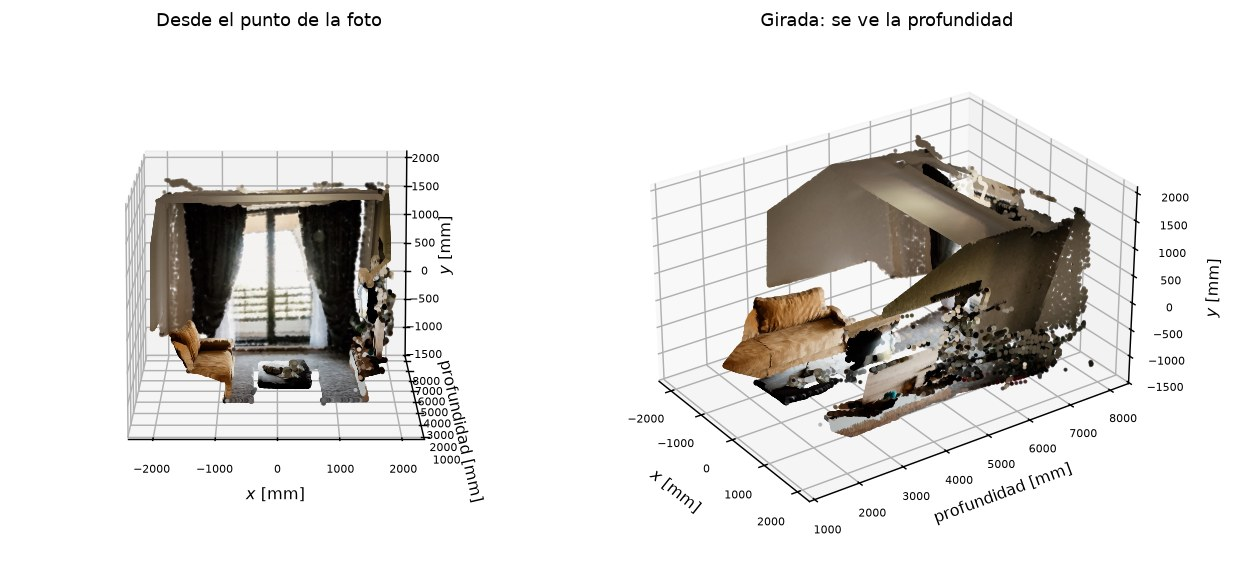
\includegraphics[width=0.97\linewidth]{hab_nube.jpg}
\caption{Vértices de la malla de la sala con el color de la foto: visto desde el punto de la foto (izquierda) y girado (derecha), donde se ve que el piso, las paredes y el techo son
planos y que el sofá y la mesa quedan delante de la pared.}
\label{fig:hab-nube}
\end{figure}

\begin{table}[htbp]
\caption{Medidas de la reconstrucción de la sala de referencia}
\label{tab:hab-res}
\centering\small
\begin{tabular}{@{}p{7.2cm}r@{}}
\toprule
Medida & Valor \\
\midrule
Píxeles de la foto & 614\,400 \\
Planos encontrados (piso, techo y 4 paredes) & 6 \\
Nodos de la rejilla de adelante & 153\,600 \\
Triángulos de la rejilla / eliminados por saltos & 305\,602 / 2\,612 (0{,}85\,\%) \\
Vértices de la capa de atrás & 42\,168 \\
Vértices $N$ y triángulos $M$ de la malla & 195\,768 y 380\,493 \\
Altura de la cámara sobre el piso & 1{,}21 m \\
Inclinación de la cámara corregida con la rotación & 3{,}36$^\circ$ \\
Dispersión de la altura del piso antes y después de girar & 67{,}6 mm y 6{,}5 mm \\
Desviación del piso respecto de su plano antes y después & 0{,}9 cm y menos de $10^{-3}$ cm \\
Tiempo total & 29{,}4 s \\
\bottomrule
\end{tabular}
\note{No hay una medida de referencia de la sala, así que estos valores muestran la coherencia interna (planitud, perpendicularidad), no el error contra el cuarto real.}
\end{table}
